\documentclass[aspectratio=169, 8pt,t]{beamer}
\graphicspath{{figures/}} % Setting the graphicspath

% Theme settings
\usetheme{Madrid}
\usecolortheme{default}
\setbeamertemplate{navigation symbols}{}   % removes navigation symbols such as 'next page'
\setbeamertemplate{footline}{}             % remove line with name, date, page nr. 
\setbeamercolor*{frametitle}{bg=white}     % remove background from frametitle
\usepackage{caption}
% \captionsetup[figure]{labelformat=empty}% redefines the caption setup of the figures environment in the beamer class.
\setbeamersize{text margin left=20pt,text margin right=10pt}
\usefonttheme[onlymath]{serif} % makes beamer math look like article math
\usepackage{hyperref}


%======================= page numbering =======================
\addtobeamertemplate{navigation symbols}{}{ \usebeamerfont{footline}
  \insertframenumber / \inserttotalframenumber \hspace*{2mm} \\ \vspace*{1mm} 
}


%=================================== colors ====================================
\definecolor{RoyBlue}{RGB}{22, 46, 69}
\definecolor{RoyGrey}{RGB}{64, 88, 128} 

\newcommand{\hlme}[1]{{\color{red}\bf #1}} % highlight me

\setbeamercolor{structure}{fg=RoyBlue} % itemize, enumerate, etc
\setbeamercolor{frametitle}{fg=RoyGrey}
\setbeamercolor{section in head/foot}{bg=RoyBlue}


%======================= add progress dots to headline =========================
\setbeamertemplate{headline}{%
    \begin{beamercolorbox}[ht=4mm,dp=4mm]{section in head/foot}
        \insertnavigation{\paperwidth}
    \end{beamercolorbox}%
}%
\makeatother


%======================= add section title page ================================
\AtBeginSection[]{
  \begin{frame}
  \vfill
  \centering
    \usebeamerfont{title}\insertsection\par%
  \vfill
  \end{frame}
}


%=================================== titlepage =================================
\title{Electroweak and QED effects in PDF determination}
\date{QCD@LHC 2023  \\[0.1cm] 4 September 2023, Durham}
\author{Roy Stegeman}
\institute{\small The University of Edinburgh}


\titlegraphic{\vspace*{6mm}
  
\includegraphics[height=1.5cm]{logos/edi_logo.png} \hspace{10mm}
  % 
\includegraphics[height=0.8cm]{logos/nnpdf_logo_official.pdf} \hspace{10mm}
  
\includegraphics[height=1.5cm]{logos/higgs_logo.jpg}
}

\defbeamertemplate{title page}{noinstitute}[1][]
{
  \vbox{}
  \vfill
  \begingroup
    \centering
    \begin{beamercolorbox}[sep=8pt,center,#1]{title}
      \usebeamerfont{title}\inserttitle\par%
      \ifx\insertsubtitle\@empty%
      \else%
        \vskip0.25em%
        {\usebeamerfont{subtitle}\usebeamercolor[fg]{subtitle}\insertsubtitle\par}%
      \fi%     
    \end{beamercolorbox}%
    \vskip2em\par
    \begin{beamercolorbox}[sep=0pt,center,#1]{author}
      \usebeamerfont{author}\insertauthor
    \end{beamercolorbox}
  \begin{beamercolorbox}[sep=0pt,center,#1]{author}
    \usebeamerfont{institute}\insertinstitute
  \end{beamercolorbox}
  \vspace*{8pt}
  \vspace*{16pt}
    \begin{beamercolorbox}[sep=0pt,center,#1]{date}
      \usebeamerfont{date}\insertdate
    \end{beamercolorbox}\vskip0.5em
    {\usebeamercolor[fg]{titlegraphic}\inserttitlegraphic\par}
  \endgroup
  \vfill
}

\makeatletter
\setbeamertemplate{title page}[noinstitute][colsep=-4bp,rounded=true,shadow=\beamer@themerounded@shadow]
\makeatother


\begin{document}
{
\setbeamertemplate{headline}{} % remove headline from titlepage
\begin{frame}
  \titlepage
\end{frame}
}

\setbeamertemplate{enumerate items}[default]

\pgfdeclarelayer{bg}    % declare background layer
\pgfsetlayers{bg,main}  % set the order of the layers (main is the standard layer)


% SLIDES =======================================================================


% Introduction:
%   - factorization
%   - status of modern PDFs: good agreement, approaching percent-level accuracy
%   - 3 necessary ingredients for the LHC precision era should be considered together: N3LO, theory uncertainty, QED

% aN3LO: % only discuss splitting functions in more detail
%   - Requirements: splitting functions, heavy-quark matching conditions, DIS coefficients, Hadronic coefficients (K-factors)
%   - Status of 4-loop splitting functions
%   - different approximation between NNPDF (with IHOU) and MSHTaN3LO (nuisance parameter), show comparison of splitting functions

% Theory uncertainties:
%   - IHOU for N3LO
%   - MHOU: scale variations are commonly used for partonic cross-sections -> use same idea to construct a covmat
%   - show plot comparing NNLO-NLO to MHOU, MHOU conservative
%   - impact of MHOU on PDF fit (show plots)
%   - compare aN3LO with IHOU&MHOU and NNLO with MHOU

% QED: % don't include discussion of DGLAP basis since that's too technical
%   - Requirements: splitting functions, photon PDF (luxQED), ideally photon initiated theory calculations
%   - discuss luxQED, modified momentum sumrule. 
%   - slightly different procedures (different initial scale choices): 
%     NNPDF: iterative procedure due to photon in MSR, 
%     MSHT20: PI contributions
%     CT18: own uncertainty estimation
%   - comparison plots: NNPDF4.0 vs NNPDF4.0QED, NNPDF4.0QED vs CT18qed vs MSHT20qed
%   - pheno plots form NNPDF4.0QED draft, high 
%   - (optional) highlight pineAPPL

% Summary and Outlook



\section*{Introduction}

% TODO: color DY schemetic corresponding to colors of equation
\begin{frame}{PDFs at hadron colliders}
  Collinear factorization enables the prediction of cross-sections
  \begin{equation*}
    \sigma_{\mathrm{LHC}}(M, s) \propto \sum_{i j} \int_{M^2}^s d \hat{s} {\color{blue}\mathcal{L}_{i j}(\hat{s}, s)} {\color{red}\hat{\sigma}_{i j}\left(\hat{s}, \alpha_s(M)\right)}, \quad i,j = \{g, u, \bar{u}, d, \bar{d}, \ldots\}
  \end{equation*}

  \begin{columns}
    \begin{column}{0.49\textwidth}
      Partonic luminosity
      \begin{equation*}
        {\color{blue}\mathcal{L}_{i j}(Q, s)}=\frac{1}{s} \int_{Q^2 / s}^1 \frac{d x}{x} {\color{teal}f_i\left(\frac{Q^2}{s x}, Q\right) f_j(x, Q)}
      \end{equation*}
      Parton Distribution Function:
      \begin{equation*}
        {\color{teal} f_j(x,Q)}
      \end{equation*}
      \begin{itemize}
        \item non-perturbative QCD
        \item extracted from experimental data
        \item universal
      \end{itemize}
    \end{column}

    \begin{column}{0.49\textwidth}
      {\color{red} $\hat{\sigma}_{i j}\left(\hat{s}, \alpha_s(M)\right)$} denotes the hard-scattering coefficient function
      \begin{itemize}
        \item calculable in perturbative QCD
        \item infrared safe
        \item independent of hadron
      \end{itemize}
      \begin{figure}
        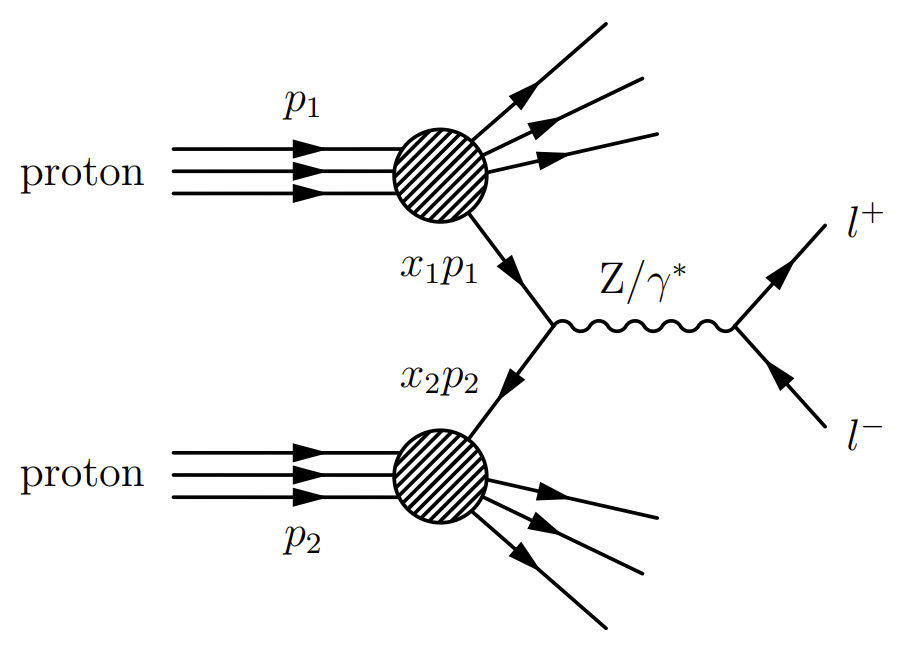
\includegraphics[width=0.5\textwidth]{figures/dy.png}
      \end{figure}
    \end{column}
  \end{columns}
\end{frame}



\begin{frame}{Status of modern PDF sets}
  PDF sets are provided by various collaborations, each using slightly different theory choices, datasets, and methodologies
  \begin{columns}
    \begin{column}{0.49\textwidth}
      \begin{figure}
        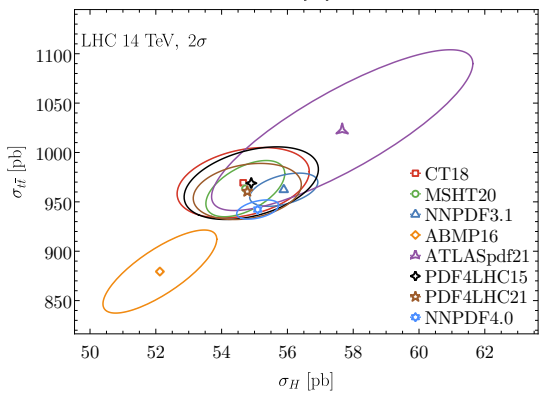
\includegraphics[width=0.7\textwidth]{Httbar_xsec}
        \caption*{\color{gray} \footnotesize [Snowmass 2021: 2203.13923]}
      \end{figure}
    \end{column}
    \begin{column}{0.49\textwidth}
      \begin{figure}
        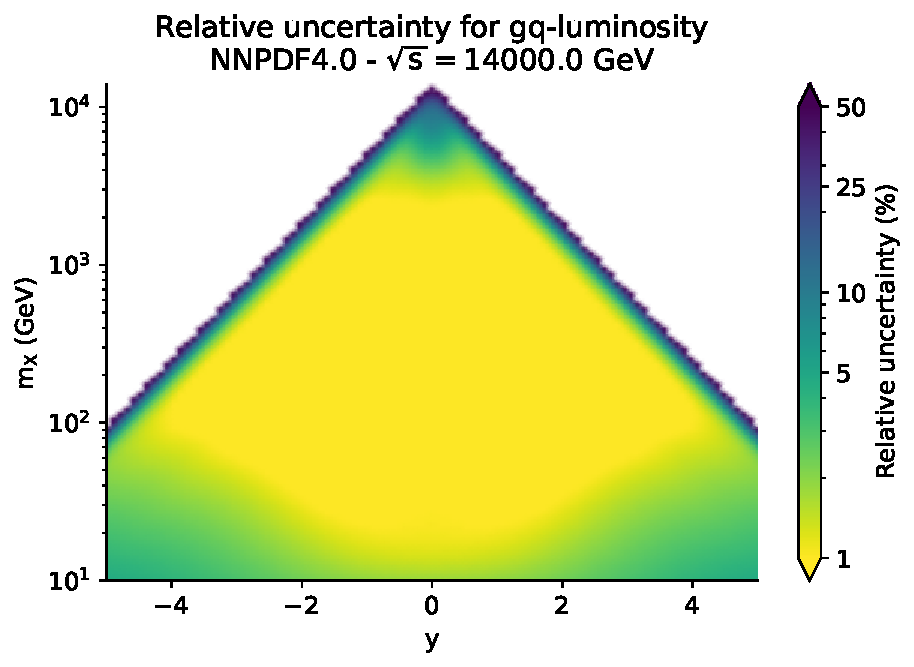
\includegraphics[width=0.7\textwidth]{gqlumi}
      \end{figure}
    \end{column}
  \end{columns}
  \begin{itemize}
  \item Results are generally consistent, but uncertainties differ
  \item Approaching percent-level accuracy
  \end{itemize}
\end{frame}


\begin{frame}{Challenges}
  PDFs, along with $\alpha_s$, are often a dominant source of uncertainty for predictions of LHC cross-sections 
  \begin{columns}
    \begin{column}{0.49\textwidth}
      \vspace*{1em}

      Requirements for the next generation of PDFs are threefold:
      \begin{itemize}
        \item To exploit the impressive progress in N3LO calculations we require PDFs of the same order
        \item Missing higher order uncertainties (MHOUs) for some observables are larger than the experimental uncertainty and can thus no longer be neglected
        \item The level of precision aimed for at the LHC no longer allows neglecting EW corrections
      \end{itemize}

      \vspace*{1em}
      Focus on QED, but briefly touch upon N3LO and MHOU

      \vspace*{0.5em}
      For details on MHOU/N3LO: Thursday's talk by Lucian Harland-Lang 
    \end{column}

    \begin{column}{0.49\textwidth}
      \begin{figure}
        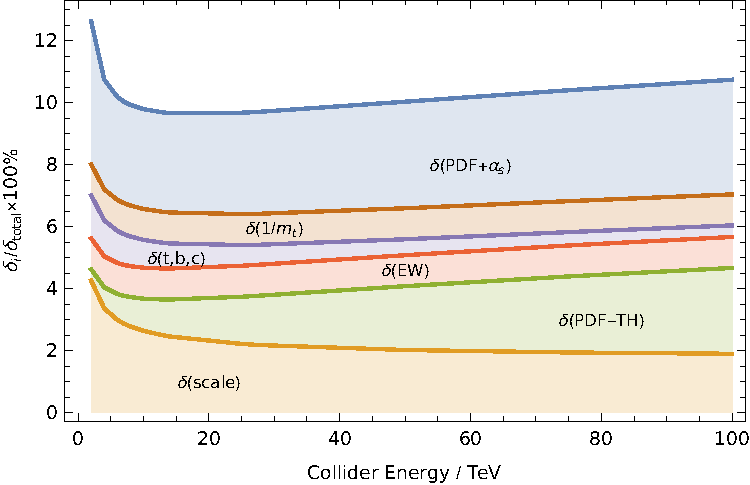
\includegraphics[width=0.8\textwidth]{figures/sources_of_unceratinty.pdf}
        \caption*{\color{gray} [HL-LHC: 1902.00134]}
      \end{figure}
    \end{column}
  \end{columns}
\end{frame}


% ==============================================N3LO===========================
\section*{Approximate N3LO PDFs}

\begin{frame}{Requirements for N3LO PDFs}
  To produce PDFs at N3LO several inputs are needed at the corresponding order:
  \begin{itemize}
    \item QCD splitting functions for DGLAP evolution
    \item Matching conditions for heavy-quark mass schemes
    \item DIS partonic coefficients 
    \item Hadronic coefficients (mainly included through K-factors)
  \end{itemize}

  \vspace*{1em}
  Not all completely available at N3LO, thus reliable approximations are needed. E.g. splitting functions:
  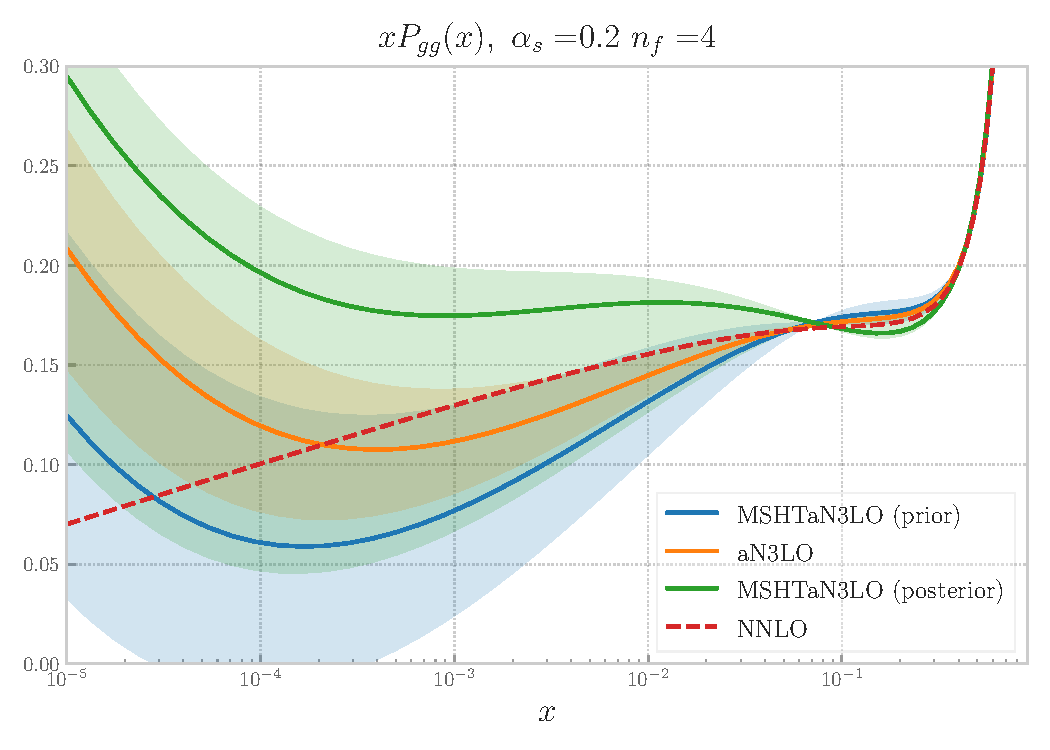
\includegraphics[width=0.29\textwidth]{figures/gamma_gg_msht_logx.pdf}
  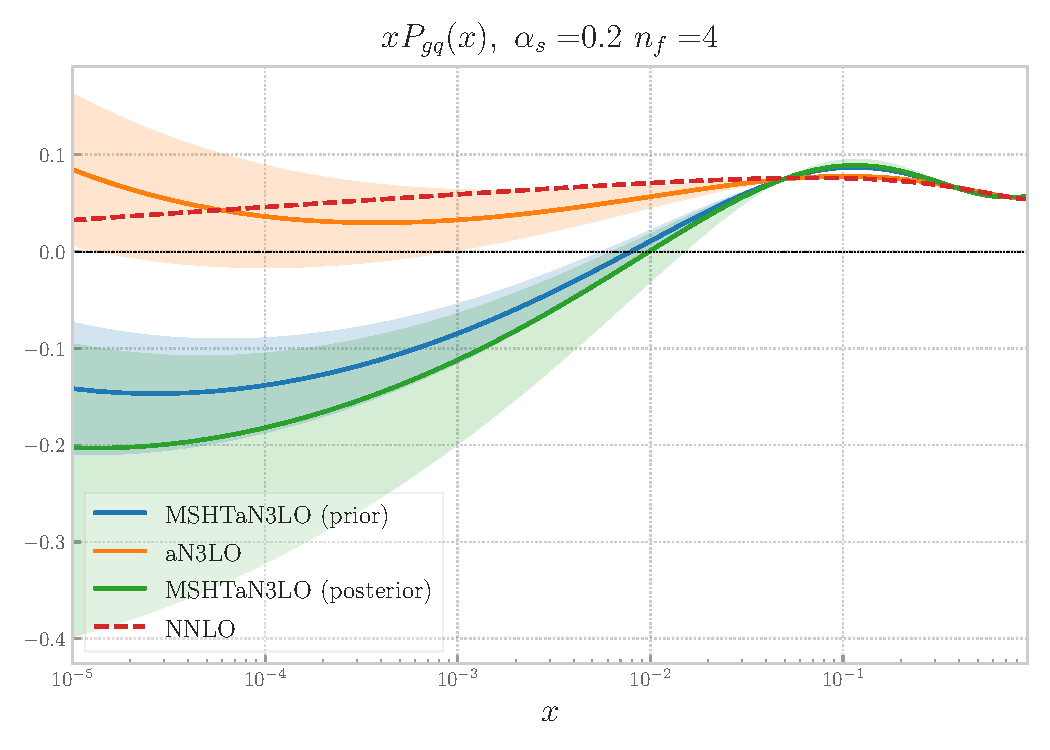
\includegraphics[width=0.29\textwidth]{figures/gamma_gq_msht_logx.pdf}
  \begin{itemize}
    \item MSHTaN3LO posterior uncertainties based on fitting nuisance parameter
    \item To avoid fitting a nuisance parameter NNPDF4.0 accounts for IHOU through covariance matrix formalism
    \item Generally good agreement except for $P_{gq}$
  \end{itemize}
\end{frame}

% \begin{frame}{4-loop splitting functions}
%   The complete N3LO splitting functions are not yet know, but a lot of information is available:
%   \begin{itemize}
%     \item Non-singlet splitting functions are estimated to quite high precision \\
%     {\color{gray} [Moch, Ruijl, Ueda, Vermaseren, Vogt: 1707.08315], [Davies, Vogt, Ruijl, Ueda, Vermaseren: 1610.07477] [Davies, Kom, Moch, Vogt: 2202.10362] }
%     \item Singlet spitting functions are more challenging, main results used for approximation are:
%     \begin{itemize}
%       \item Large-$n_f$ limit: {\color{gray} [Davies, Vogt, Ruijl, Ueda, Vermaseren: 1610.0744]}
%       \item Small-x limit: {\color{gray} [Bonvini and Marzani: 1805.06460] [Davies, Kom, Moch, Vogt: 2202.10362]}
%       \item Large-x limit: {\color{gray} [Duhr, Mistlberger, Vita 2205.04493], [Henn, Korchemsky, Mistlberger: 1911.10174], [Soar, Moch, Vermaseren, Vogt: 0912.0369]}
%       \item Mellin Moments: {\color{gray} [Falcioni, Herzog, Moch, Vogt: 2302.07593, 2307.04158], [Moch, Fuijl, Ueda, Vermaseren, Vogt: 2111.15561]}
%     \end{itemize}
%   \end{itemize}

%   \begin{itemize}
%     \item Different functions can be used to combine known moments and results, this has a corresponding incomplete higher order uncertainty (IHOU)
%     \item So far only MSHTaN3LO is available, NNPDF4.0aN3LO coming soon!  
%   \end{itemize}
% \end{frame}


% \begin{frame}{Comparison of aN3LO splitting functions}
%   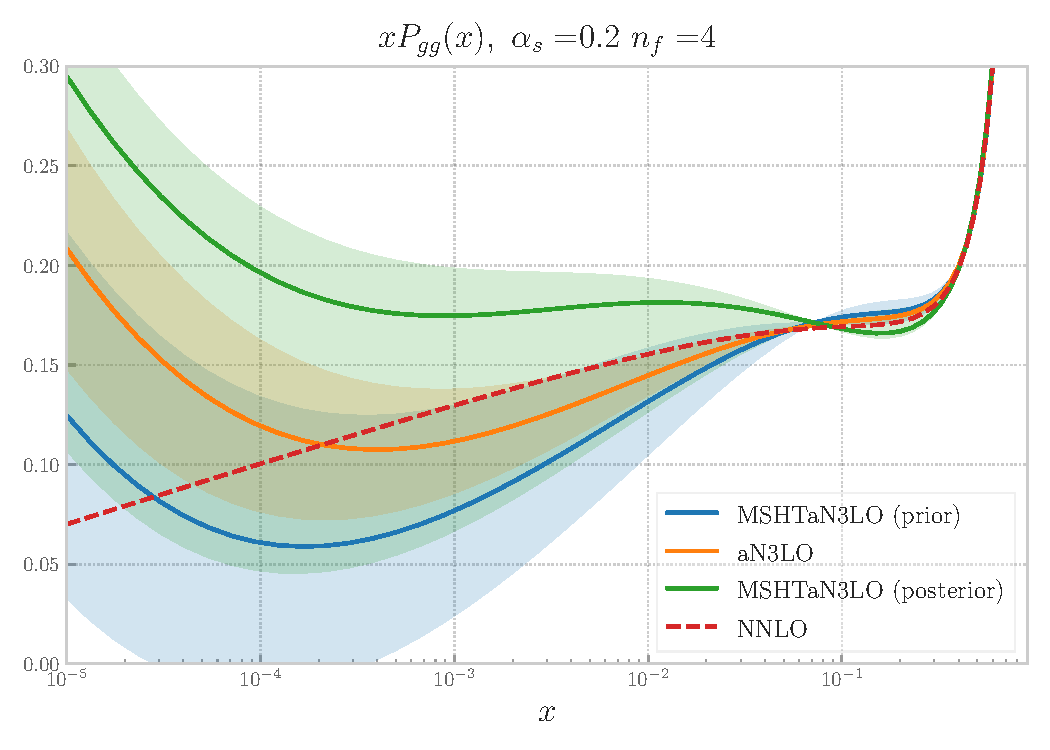
\includegraphics[width=0.39\textwidth]{figures/gamma_gg_msht_logx.pdf}
%   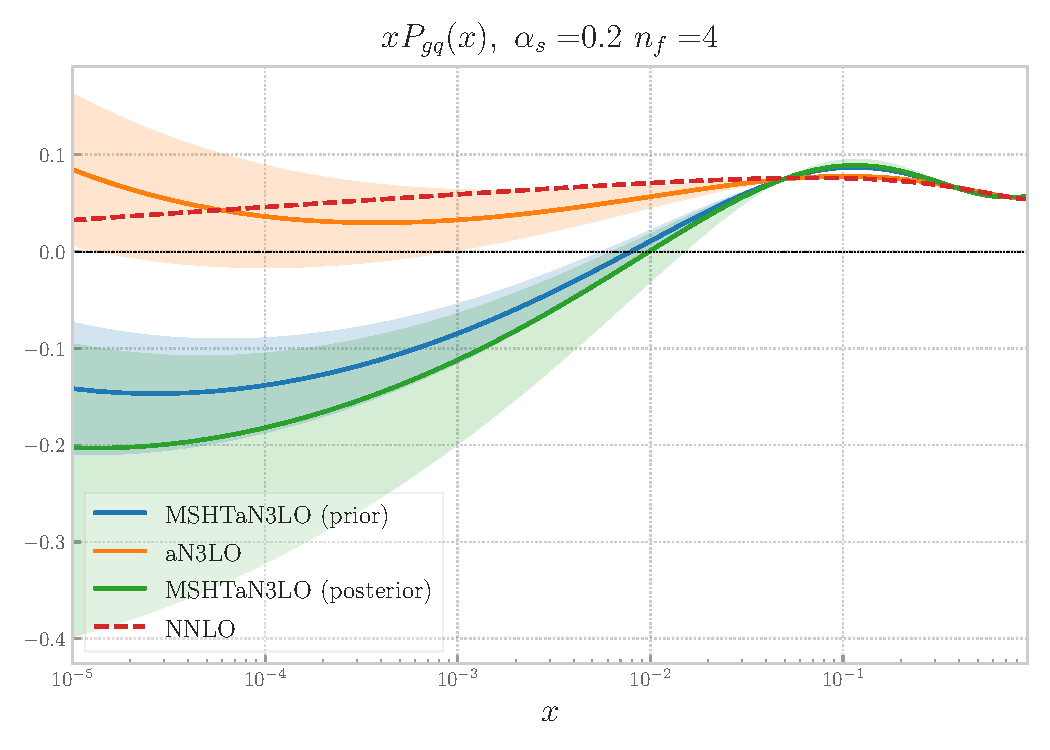
\includegraphics[width=0.39\textwidth]{figures/gamma_gq_msht_logx.pdf}
%   \begin{itemize}
%     \item MSHTaN3LO posterior uncertainties based on fitting nuisance parameter
%     \item To avoid fitting a nuisance parameter NNPDF4.0 accounts for IHOU through covariance matrix formalism
%     \item Generally good agreement except for $P_{gq}$
%   \end{itemize}
% \end{frame}


% ========================================Theory uncs===========================

\section*{Missing higher order uncertainties}

\begin{frame}{Missing higher order uncertainties}
  \begin{columns}[T]
    \begin{column}{0.49\textwidth}
      \begin{itemize}
        \item Partonic cross sections and DGLAP splitting functions are computed perturbatively and thus have a corresponding uncertainty to the neglected higher orders
        \item Higher order uncertainties are generally estimated through variation of the unphysical renormalization (for partonic cross-sections) and factorization (for anomalous dimensions) scales
        \item MHOUs are included through the covariance matrix formalism as previously done in NNPDF3.1 {\color{gray} [NNPDF: 1906.10698]}
        \item This assumes the experimental and theoretical uncertainties are Gaussian and independent
      \end{itemize}
    \end{column}
    \begin{column}{0.49\textwidth}
      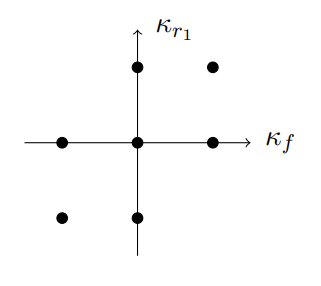
\includegraphics[width=0.89\textwidth]{figures/7ptsv.png}
    \end{column}
  \end{columns}
\end{frame}

\begin{frame}{Validating MHOU}
  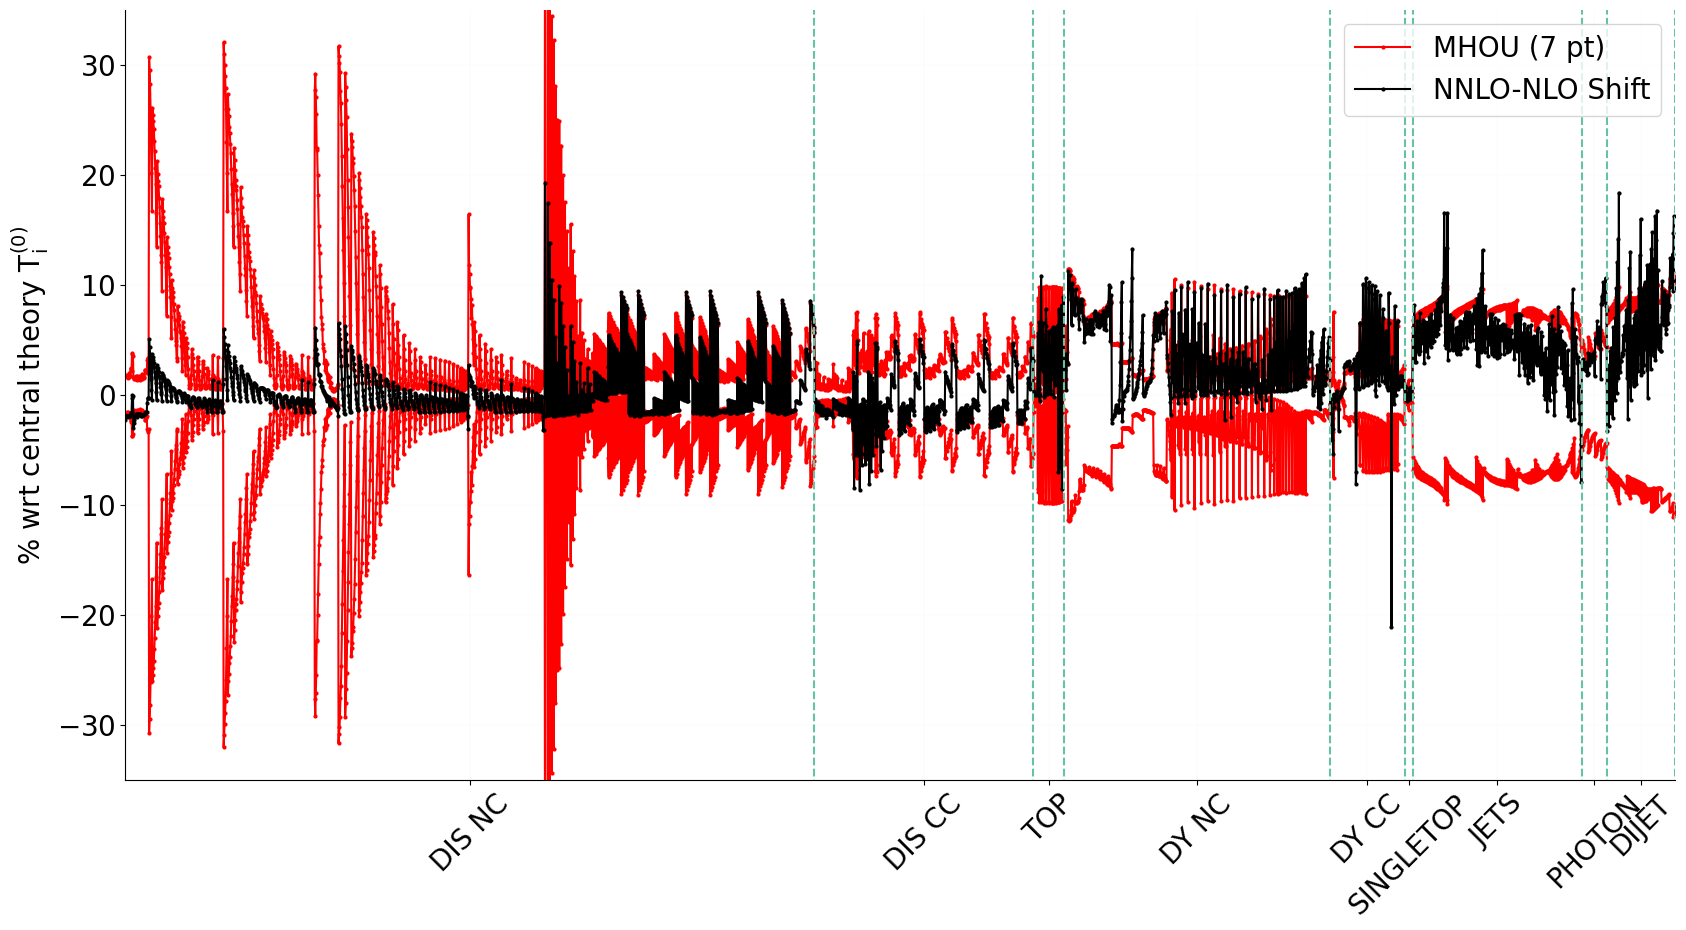
\includegraphics[width=0.69\textwidth]{figures/shift_validation.png}

  We can test the NLO MHOU and observe that generally MHOU are faithfully estimated while conservative for DIS
\end{frame}

% \begin{frame}{Impact of MHOU on PDF}
% \end{frame}

% \begin{frame}{Impact of MHOU on Pheno}
% \end{frame}

% ========================================QED===================================
\section*{QED corrections}

\begin{frame}{Including QED corrections in a PDF set}
  The current standard for PDFs determination is at NNLO in QCD, however  $\alpha(M_z) \sim \alpha_s^2(M_Z)$

  \begin{columns}
    \begin{column}{0.49\textwidth}

      \vspace*{1em}
      Including QED corrections in PDFs consists of \vspace*{0.5em}
      \begin{itemize}
        \item QED corrections to DGLAP (at $\mathcal{O}(\alpha)$, $\mathcal{O}(\alpha \alpha_s)$ and $\mathcal{O}(\alpha^2))$: \\ 
        $P_{QED}=\alpha P_{ij}^{(0,1)}+\alpha \alpha_s P_{ij}^{(1,1)}+\alpha^2 P_{ij}^{(0,2)}+\ldots$
        \vspace*{0.5em}
        \item Adding a photon PDF and including photon initiated contributions to cross-sections \\
        The momenum sumrule is modified accordingly:   
        \begin{equation*}
          \int_0^1 dx\, \left(  x\Sigma(x,Q^2) + xg(x,Q^2) + x\gamma(x,Q^2) \right) =1
        \end{equation*}
      \end{itemize}
    \end{column}

    \begin{column}{0.49\textwidth}
      \begin{figure}
        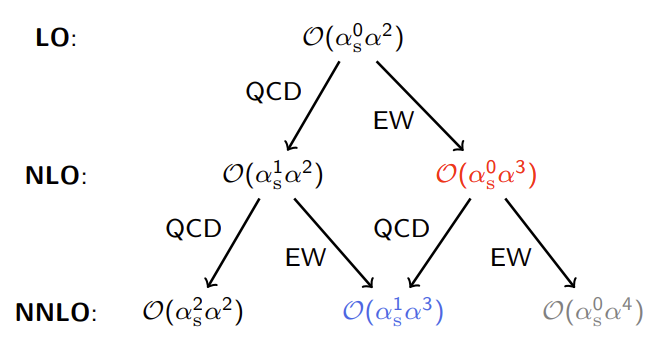
\includegraphics[width=0.99\textwidth]{figures/ewcorrections_dy.png}
        \caption*{Example: EW corrections in DY}
      \end{figure}
    \end{column}
  \end{columns}
\end{frame}


\begin{frame}{Determination of the photon PDF}
  Initially the photon PDF was included in a model-dependent way, however with the LUXqed approach it can be computed perturbatively {\color{gray} [Manohar, Nason, Salam, Zanderighi: 1607.04266]}
  \begin{columns}[T]
    \begin{column}{0.59\textwidth}
      \begin{equation*}
        \begin{split}
          & x \gamma(x, \mu^2)
          =
          \frac{2}{\alpha (\mu^2)} \int\limits_x^1 \frac{dz}{z}
          \Biggl\{ \int_{m_p^2x^2 \over 1-z}^{\mu^2 \over 1-z} \frac{dQ^2}{Q^2}
          \alpha^2(Q^2) \Biggl[ -z^2 F_L(x/z, Q^2) \\
          & + \left( z P_{\gamma q}(z) + \frac{2 x^2 m_p^2}{Q^2} \right)
          F_2(x/z, Q^2)\Biggr] - \alpha^2(\mu^2) z^2 F_2(x/z, \mu^2)\Biggr\}
        \end{split}
      \end{equation*}
      LUXqed has been used in all of the most recent QED PDFs:
      \begin{itemize}
        \item MMHT2015qed
        \item NNPDF3.1QED
        \item CT18QED
        \item MSHT20QED
        \item Soon: NNPDF4.0QED
      \end{itemize}
    \end{column}

    \begin{column}{0.39\textwidth}
      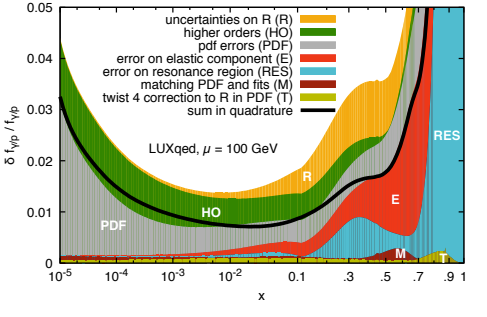
\includegraphics[width=0.99\textwidth]{figures/luxQED_uncs.png}
    \end{column}
  \end{columns}
\end{frame}

\begin{frame}{The photon PDF by different groups}
  \begin{columns}
    \begin{column}{0.59\textwidth}
      Details of the, implementation and correspondingly the above equation, vary between PDF fitting groups:

      \vspace*{1em}
      The input scale $Q_0$
      \begin{itemize}
        \item 1 GeV for MSHT20
        \item 3(1.3) GeV for CT18qed(1.3GeV)
        \item No evolution or sumrule for CT18lux
        \item 100 GeV for NNPDF4.0
      \end{itemize}

      \vspace*{1em}
      MSHT20 modifies the LUXqed formula accordingly

      \vspace*{1em}
      CT18qed initializes the photon at an input scale and evolves using DGLAP, while CT18lux calculates the photon at all scales

      \vspace*{1em}
      NNPDF3.1QED and NNPDF4.0QED use an iterative procedure to address the interplay between the photon and other PDFs due to the momentum sumrules
    \end{column}

    \begin{column}{0.39\textwidth}
      \vspace*{-1.5em}
      \begin{figure}
        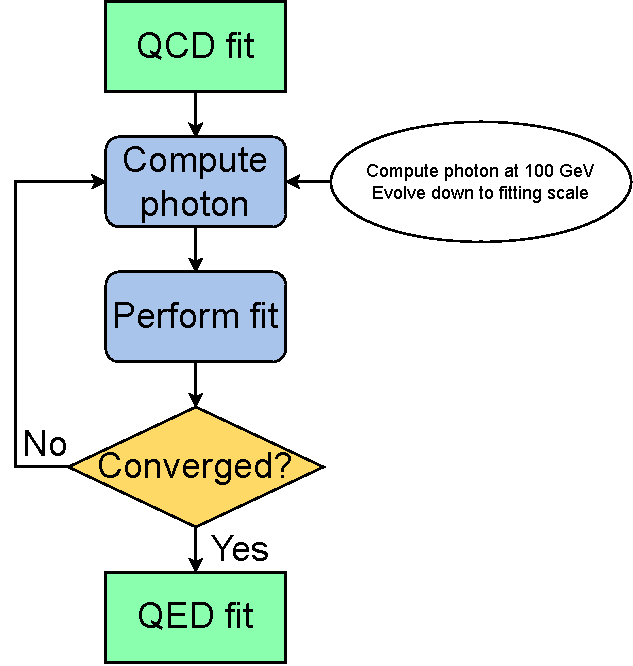
\includegraphics[width=0.9\textwidth]{figures/luxqed_iteration.pdf}
        \caption*{\color{gray} [NNPDF3.1QED: 1712.07053]}
      \end{figure}
    \end{column}
  \end{columns}

\end{frame}


\begin{frame}{Impact of the photon on other PDFs}
  \begin{center}
    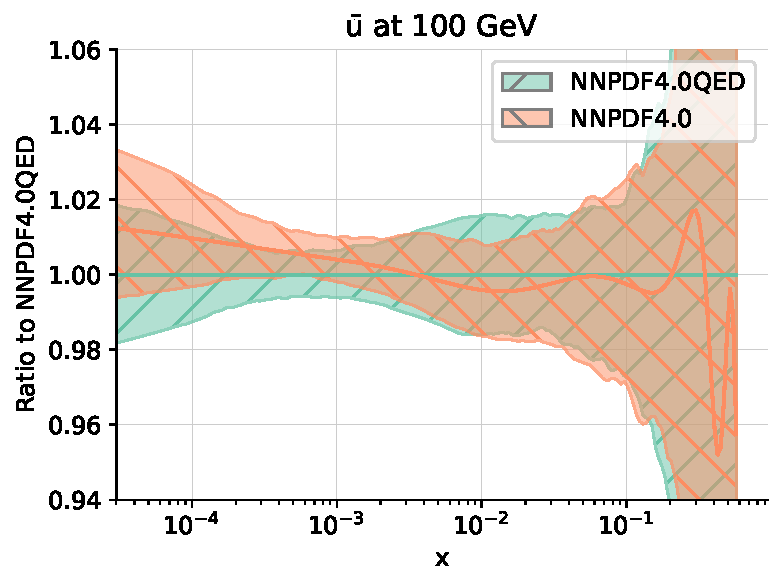
\includegraphics[width=0.45\textwidth]{figures/nnpdf40_vs_qed_ubar.pdf}
    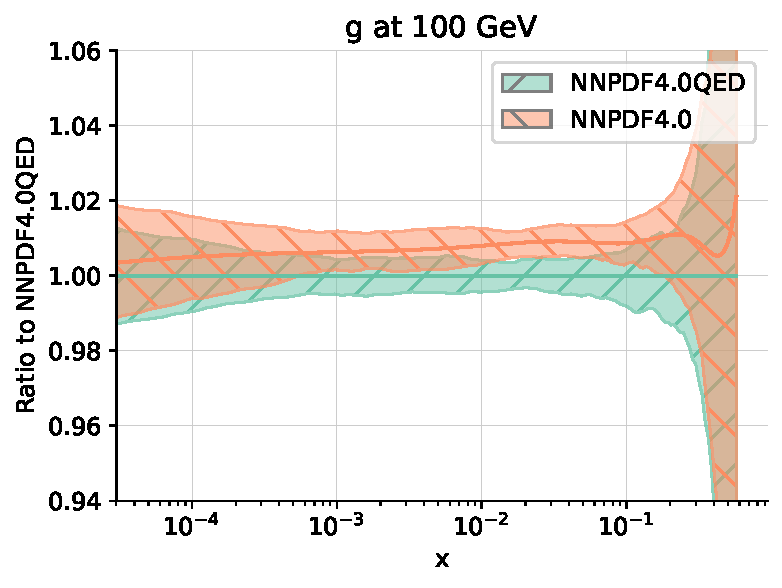
\includegraphics[width=0.45\textwidth]{figures/nnpdf40_vs_qed_g.pdf}
  \end{center}
  \begin{itemize}
    \item PDFs are in agreement within uncertainty
    \item Largest impact on the gluon due momentum transfer to the photon
  \end{itemize}
\end{frame}


\begin{frame}{QED PDF results}
  \begin{center}
    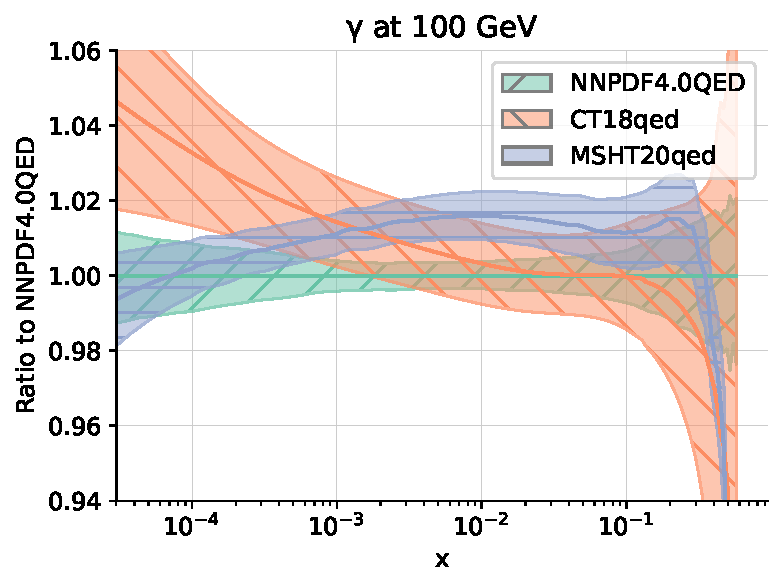
\includegraphics[width=0.3\textwidth]{figures/photon_comparison.pdf}
    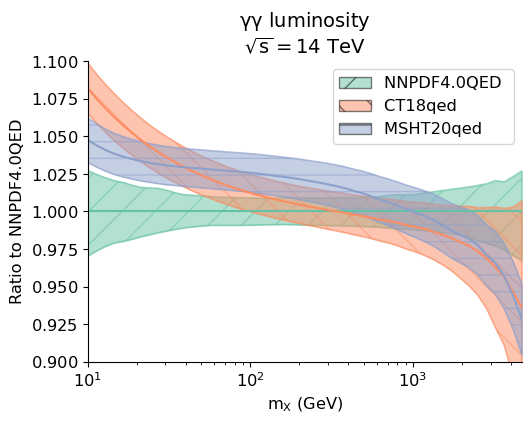
\includegraphics[width=0.3\textwidth]{figures/pp_lumi_comparison.png}
    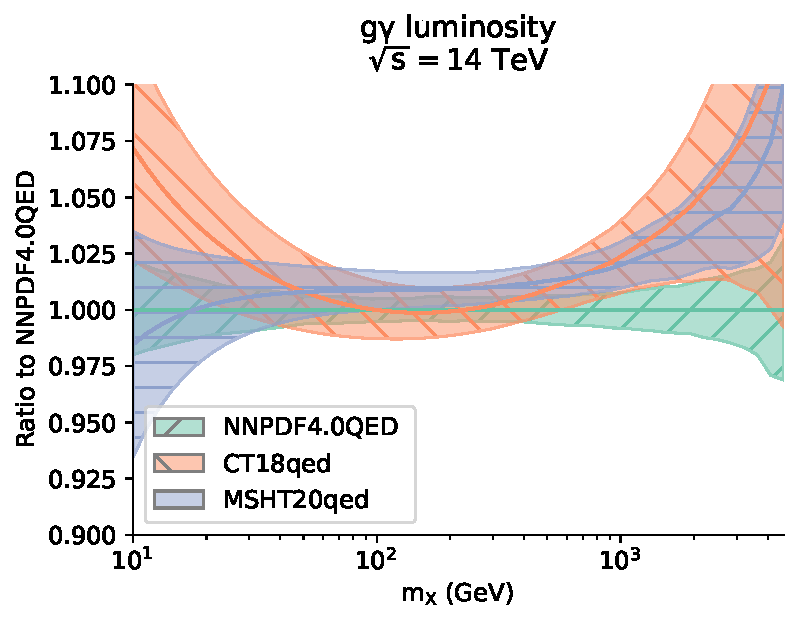
\includegraphics[width=0.3\textwidth]{figures/gp_lumi_comparison.pdf}
  \end{center}
  \begin{itemize}
    \item Because all groups use the luxQED formalism, the photon PDFs agree at percent level despite larger disagreement between other PDFs
    \item Luminosity differ only at very small and very large invariant mass
  \end{itemize}
\end{frame}


\begin{frame}{Phenomenological impact of QED effects}
  \begin{columns}[T]
    \begin{column}{0.49\textwidth}
      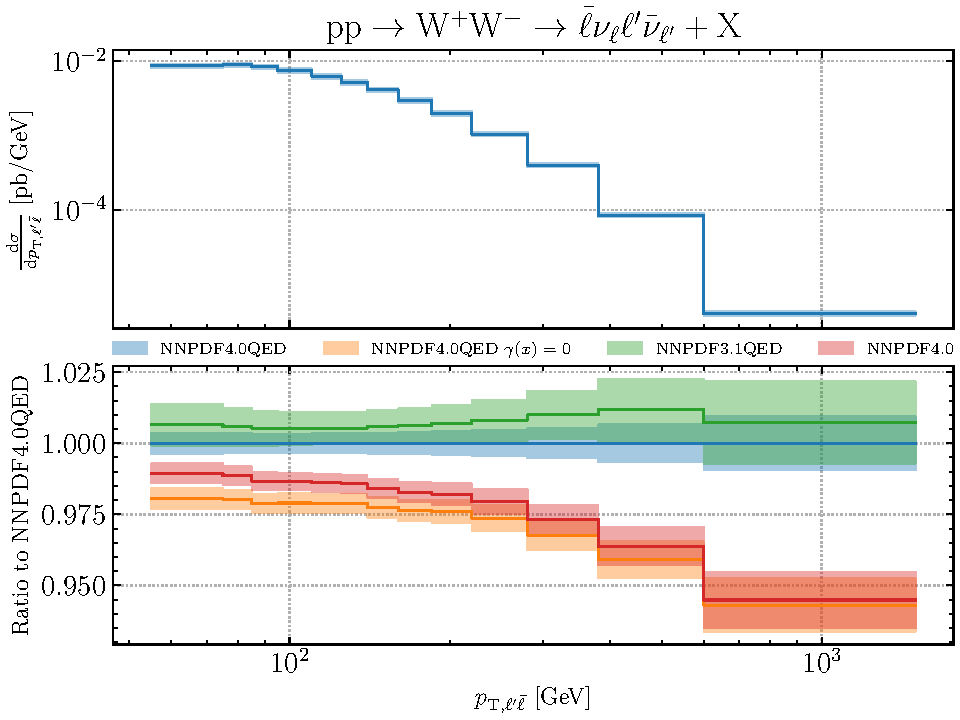
\includegraphics[width=0.7\textwidth]{figures/NNPDF_WPWM_14TEV_40_PHENO-internal.pdf}
    \end{column}
    \begin{column}{0.49\textwidth}
      \vspace*{-3.5em}
      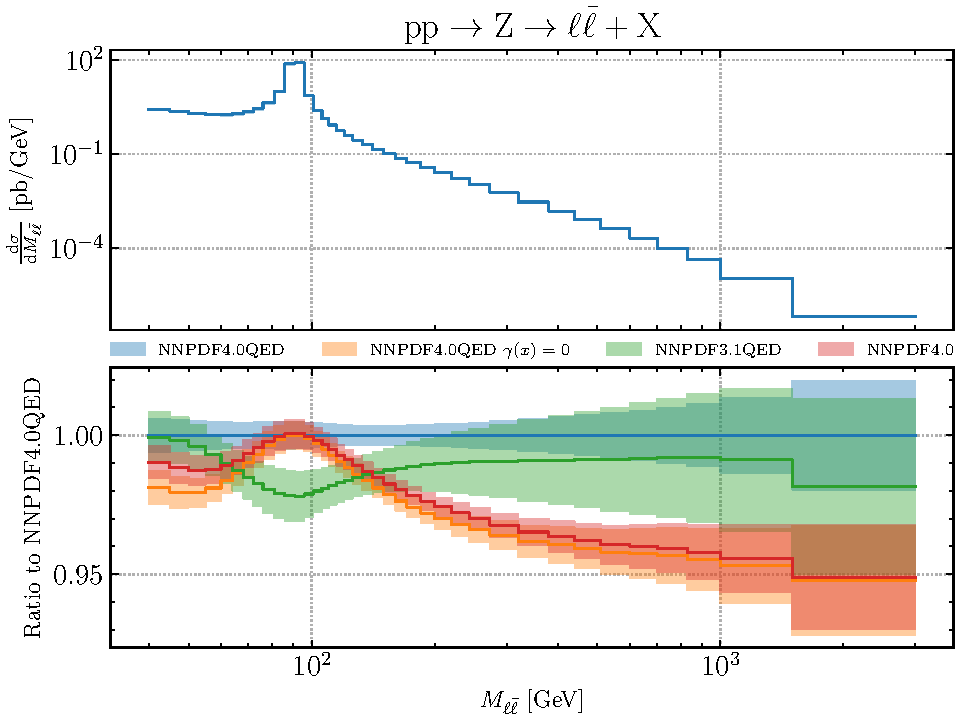
\includegraphics[width=0.7\textwidth]{figures/NNPDF_DY_14TEV_40_PHENO-internal.pdf}
    \end{column}
  \end{columns}
  \begin{columns}[T]
    \begin{column}{0.49\textwidth}
      \vspace*{1em}
      \begin{itemize}
        \item Here photon initiated contributions are included
        \item Non-negligable QED corrections in the large invariant mass and large-$p_T$ regions
        \item Percent-level enhancement near the $Z$-peak
        % \item Results produced using PineAPPL grids
      \end{itemize}
    \end{column}
    \begin{column}{0.49\textwidth}
      \vspace*{-3em}
      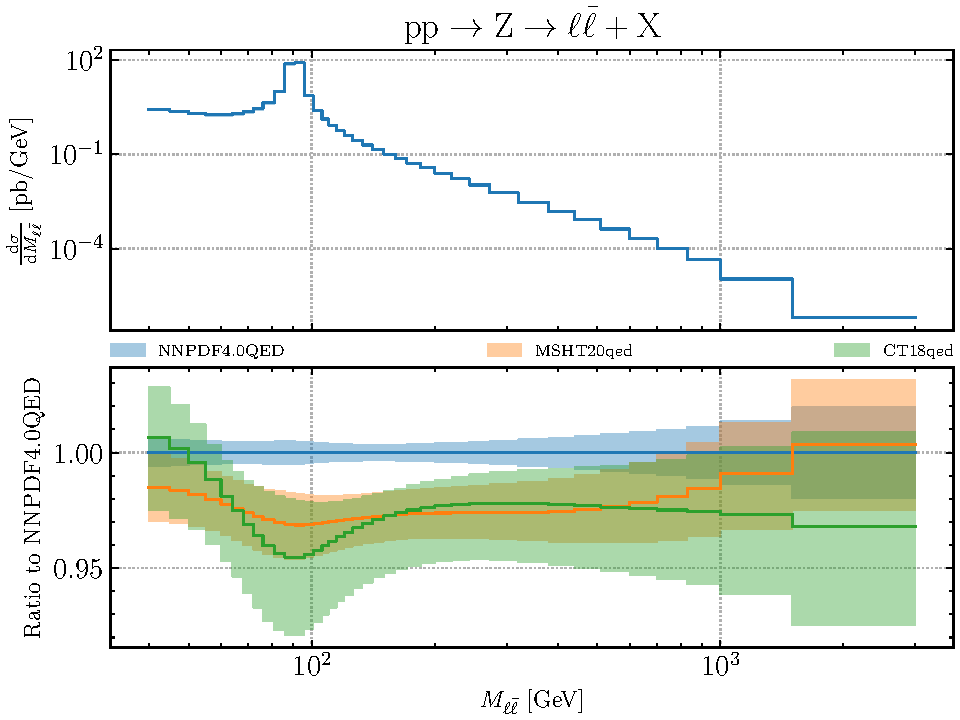
\includegraphics[width=0.7\textwidth]{figures/NNPDF_DY_14TEV_40_PHENO-global.pdf}
    \end{column}
  \end{columns}
\end{frame}


% ===============================Summary and outlook============================
\section*{Summary and outlook}

\begin{frame}{Summary and outlook}

  \begin{columns}[T]
    \begin{column}{0.49\textwidth}
      \vspace*{1em}
      Interpretation of collider measurements depends on accurate and precise theory predictions
    
      \vspace*{1em}
      The last years have seen impressive progress in N3LO calculations for LHC processes, to exploit this we need N3LO PDFs
    
      \vspace*{1em}
      Electroweak effects can no longer be neglected thus include QED corrections in DGLAP and include a photon PDF
    
      \vspace*{1em}
      The target of faithful 1\% uncertainty will require including EW effects, MHOU, and N3LO!    
    \end{column}
    \begin{column}{0.49\textwidth}
      \begin{figure}
        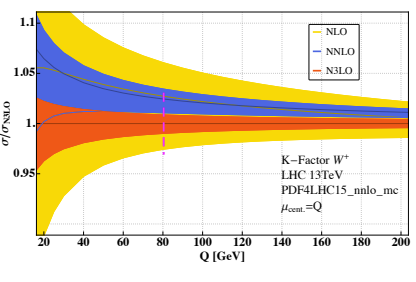
\includegraphics[width=0.9\textwidth]{figures/n3lomistlberger.png}
        \caption*{\color{gray} [Duhr, Dulat, Mistleberger 2007.13313]}
      \end{figure}
    \end{column}
  \end{columns}

  \vspace*{2em}
  \only<2>{
  \begin{center}
      {\Large \textbf{Thank you for listening!}}
  \end{center}
  }
\end{frame}


\end{document}
